Afin d'atteindre les objectifs définis par le cahier des charges du stage, le travail a été réalisé en plusieurs étapes.

\subsubsection{Documentation}
Fund KIS avait déjà repéré les technologies à utiliser pour réaliser la mission du stage. Il s'agit notamment de \href{https://getkong.org}{Kong} \footnote{voir \url{https://getkong.org}}, un \textit{API Gateway} open-source c'est-à-dire un gestionnaire d'API ; \href{https://swagger.io}{Swagger} \footnote{voir \url{https://swagger.io}}, un \textit{framework OAS (OpenAPI Specification)} pour gérer la documentation d'API et \href{https://www.docker.com}{Docker} \footnote{voir \url{https://www.docker.com}}, un gestionnaire de \textit{containers}. Au début du stage nous ne connaissions pas précisément à quoi servait chacun de ces différents outils. Nous nous sommes alors documentés sur chacunes de ces technologies ; c'était la première phase de la documentation. La suite a consité à étudier comment les utiliser pour réaliser notre travail.

\vspace{3mm}

Docker est déjà utilisé par Fund KIS pour le déploiement de ses applications dans des \textit{containers} en production. Un \textit{container} permet d'encapsuler une application en un format qui lui permet de tourner de façon indépendante. On peut le voir comme une machine virtuelle mais il n'est lié à aucun système d'exploitation. Il contient juste les bibliothèques et les paramètres permettant à l'application de tourner toute seule. Cela permet de s'assurer que l'application tournera quel que soit l'endroit où il est déployé puisque c'est un système complètement autonome qui contient tout ce dont il a besoin pour fonctionner.

\vspace{3mm}

Swagger est un \textit{framework} qui permet de suivre une certaine spécification pour gérer la documentation des API. Il permet d'expliquer simplement dans la documentation l'architechture \textit{RESTful} de l'API en détaillant les ressources et les opérations qu'on peut utiliser sur l'API. En utilisant \href{https://github.com/Surnet/swagger-jsdoc}{swagger-jsdoc}, on peut écrire toute la documentation de l'API comme commentaires dans le code source de l'API ; ceci est très intéressant car il permet d'avoir une documentation synchrone avec l'évolution de l'API. Les aspects concernant l'automatisation des documentations des API ont été traités par la deuxième statgiaire avec qui j'ai travaillé.

\vspace{3mm}

Kong est un \textit{API Gateway} et permet de gérer les problématiques de sécurité, d'authentification et de limites d'utilisations des API. On trouvera à la figure 1 suivante un schéma représentant le fonctionne de Kong et des \textit{API Gateway} en général. Il propose une interface \textit{RESTful} et utilise une architecture très modulaire en utilisant des \textit{plugins}. Ainsi on peut le configurer à souhait en utilisant seulement les \textit{plugins} dont on a besoin. On peut même écrire ses propres \textit{plugins} mais il faut pour cela maitriser Lua (langage de programmation).

\begin{figure}[!h]
\centering
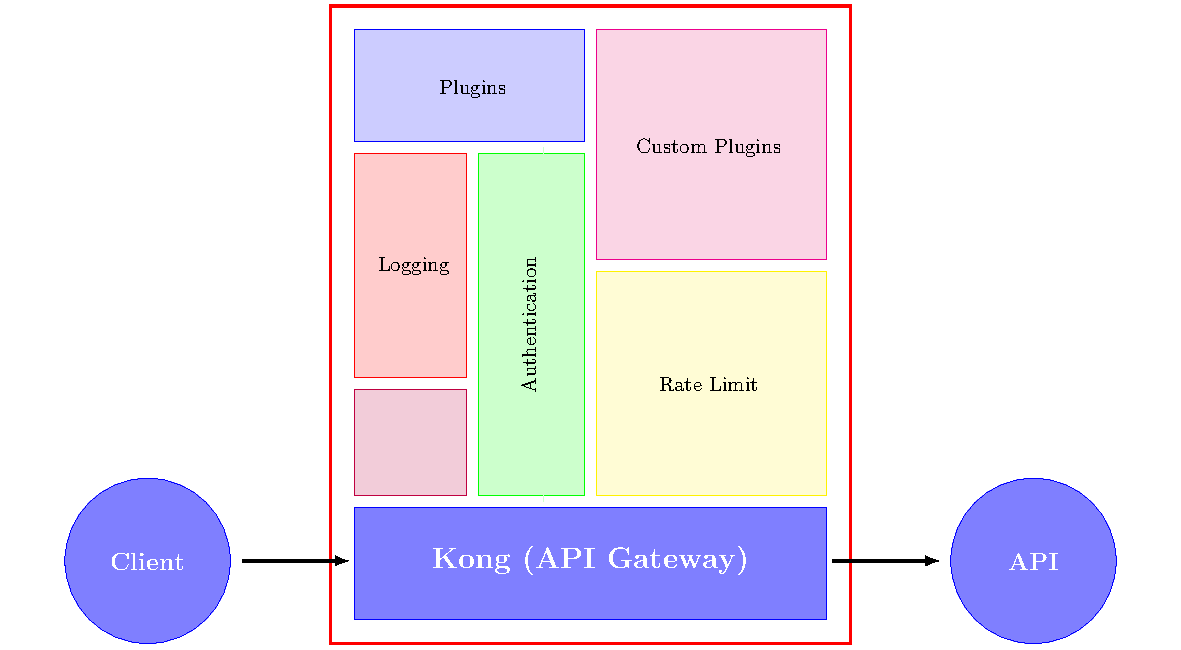
\includegraphics[width=\linewidth]{apigateway}
\caption{Structure d'un \textit{API Gateway}}
\end{figure}

\vspace{3mm}

Cependant, Kong impose une grosse contrainte : il faut absolument une base de données \textit{Cassandra} pour l'utiliser. Mais Fund KIS utilise des bases de données Mongo et SQL. Utiliser Kong comme gestionnaire d'API reviendrait à copier des données des bases données déjà utilisées par l'entreprise dans la bases de données \textit{Cassandra} que Kong va utiliser. Cela est est fastidieux et risque de poser des problèmes d'inconsistance lorsque des données sont mises à jour dans les bases. Même si Kong semblait être une solution adapté à nos problématiques, nous avons dû nous en passer.



\subsubsection{\textit{Rate limiter}}
Comme nous ne pouvons pas utiliser Kong pour gérer les API, il a été décidé de développer tout ce qu'il faut pour gérer les API. Le plus important étant un un \textit{rate limiter} : un gestionnaire de limites d'utilisations. Nous avons utilisé une \textbf{architecture microservices} car cette architecture, contrairement à une \textbf{architecture monolithique}, possède de nombreux avantages pratiques. Elle permet de décomposer une grosse application en de petites applications : en fait ces petites applications sont les composantes de la grosse application mais peuvent tourner de façon autonome. La communication entre ces différents composants peut être effecuée par différents moyen, comme des requêtes par exemple. En pratique, plusieurs personnes peuvent travailler au développement de la grosse application en s'occupant des différentes petites applications simultanément de façon beaucoup plus flexible que dans une architecture monolithique. De plus, on peut facilement réutiliser les petites applications dans d'autres grosses application. C'est comme construire différents éléments avec des blocs de lego. C'est une architecture qui est déjà largement utilisée par Fund KIS. Cela me convenait parfaitement pendant mon stage car nous travaillions à deux sur le même sujet. On peut se faire une idée rapide de la différence entre ces deux architectures en consultant les figures 2 et 3.

\begin{figure}[!h]
\centering
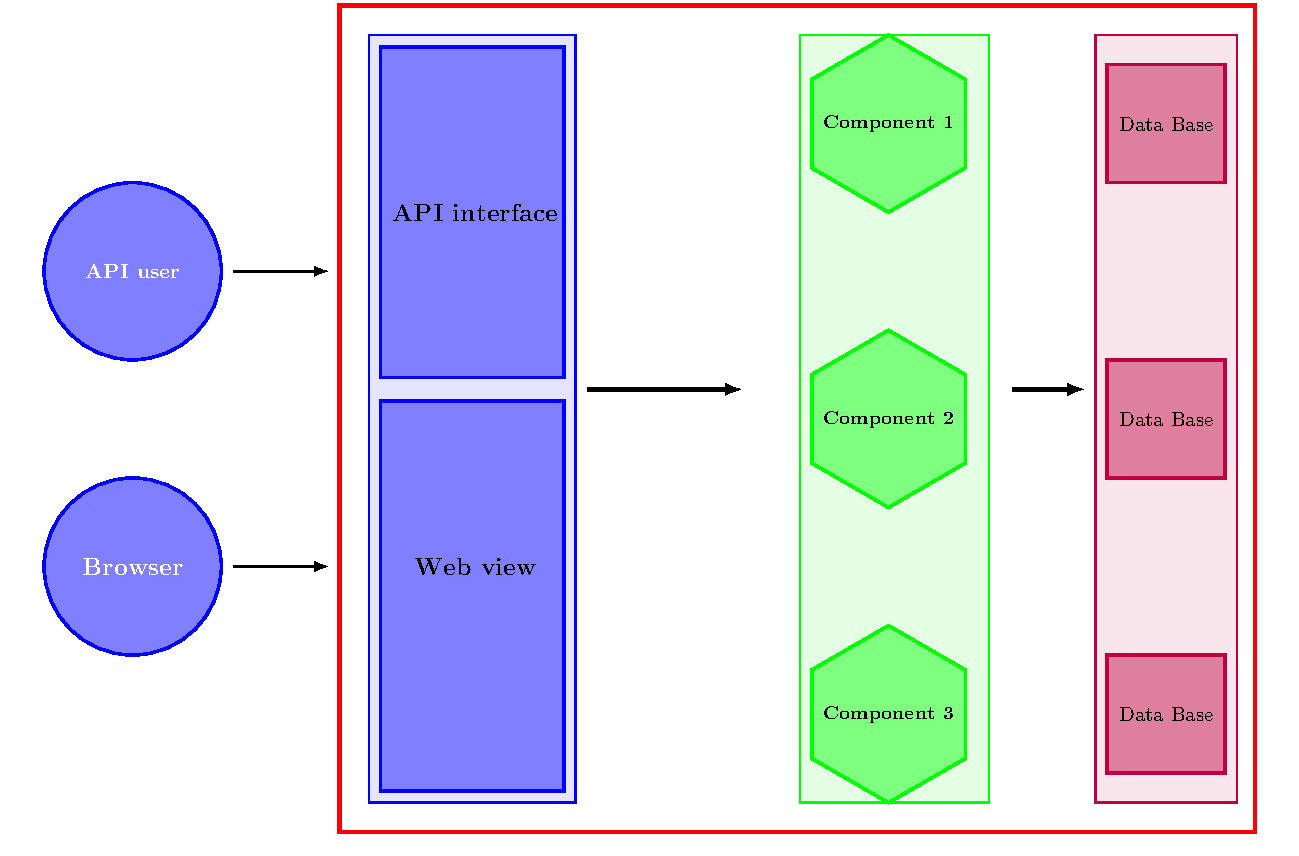
\includegraphics[width=\linewidth]{monolithique}
\caption{Architecture monolithique}
\end{figure}

\begin{figure}[!h]
\centering
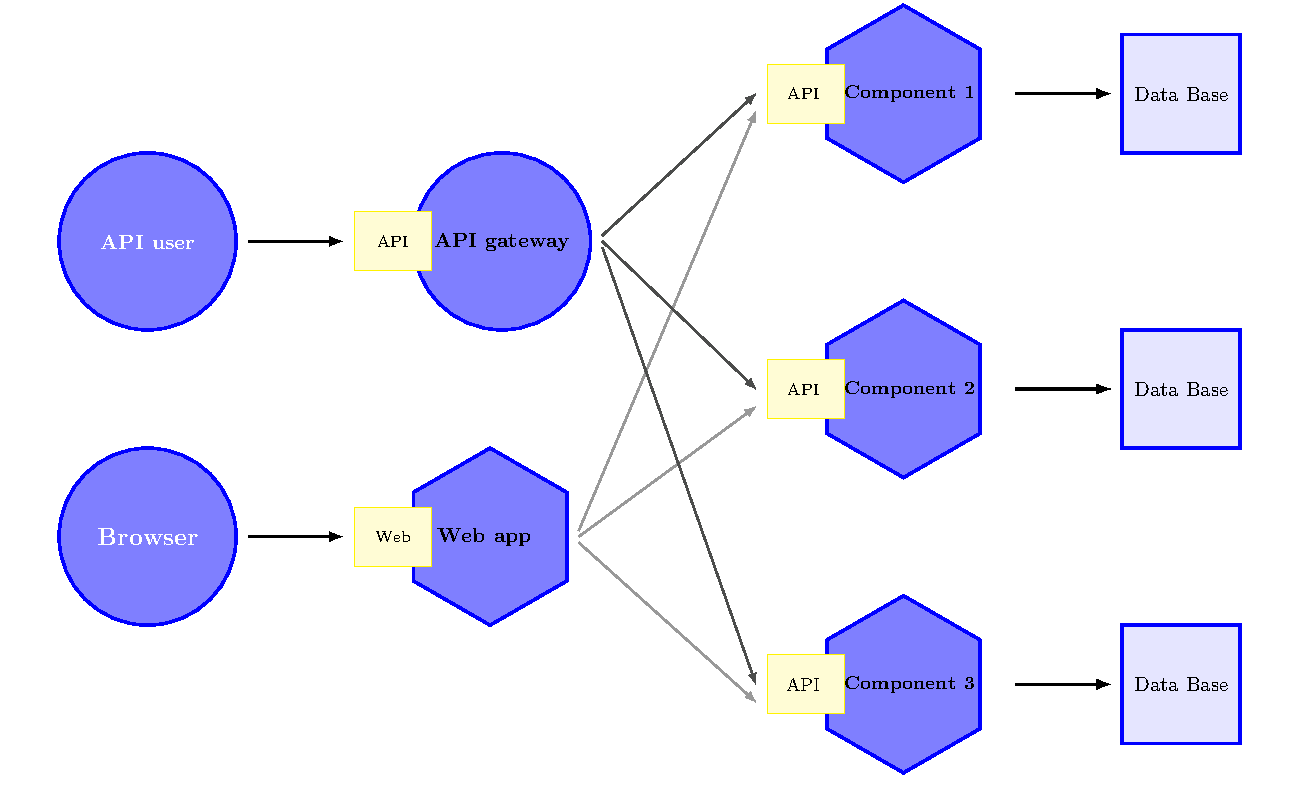
\includegraphics[width=\linewidth]{microservices}
\caption{Architecture microservices}
\end{figure}

\vspace{3mm}

L'objectif du \textit{rate limiter} est de limiter, comme l'indique son nom, le nombre d'appels qu'un utilisateur peut effectuer sur une API pendant une période de temps donnée. Cela permet d'éviter les appels intempestifs pour ne pas ralentir inutilement les serveurs. Mais l'utilisation la plus importante est l'association d'un certain nombre d'appels par période de temps aux utilisateurs selon leurs configurations. Le \textit{rate limiter} que j'ai écrit utilise l'algorithme du seau à jetons fonctionne comme suit :
\begin{itemize}[font=\color{blue}, label=\ding{43}]
  \item chaque type d'utilisateur possède un seau qui lui est associé, avec un certain nombre de jetons ;
  \item lorsqu'un utilisateur essaye d'appeler un API, on vérifie s'il possède un seau qui lui est associé et on consulte le nombre de jetons restant dans le seau ;
  \item le nombre de jetons dans le seau dépend de l'API appelée, chaque type utilisateur a donc un seau par API ;
  \item si le seau est vide, l'appel est bloqué car l'utilisateur a dépassé ses limites ;
  \item sinon, on enlève un jeton du seau et l'appel est autorisé ;
  \item le seau est crée lorsque l'utilisateur appelle une nouvelle API pour la première fois (première fois au sens où il n'y a pas de seau associé à l'utilisateur pour cette API) ;
  \item tout seau plus vieux qu'une période de temps donnée (définie par le \textit{rate limiter}) est automatiquement supprimé ; possible grâce à la fonctionnalité TTL (\textit{Time To Live}) de la base de données utilisée pour stocker les seaux : Mongodb.
\end{itemize}

\vspace{3mm}

Pour déterminer le seau à consulter lorsqu'un appel est effectué sur un API, il faut déterminer le type d'utilisateur qui a lancé l'appel. On commence par vérifier si l'utilisateur est authentifié, ce qu'il peut faire grâce une \textit{API Key}. S'il n'est pas authentifié, on utilise son \textbf{adresse IP} comme identifiant et une limite d'utilisation de l'API appelée est appliquée pour déterminer le seau. S'il est authentifié, son \textbf{id} est utilisé comme identifiant et une autre limite d'utilisation est appliquée pour l'API appelée. On a aussi laissé la possibilité qu'un utilisateur arrive ses limites d'ulisation (limites déterminées par une autre logique, un gestionnaire d'abonnements par exemple), auquel cas ces limites seront utilisées pour constituer le seau. Les différentes limites d'utilisations sont regroupées dans un fichier de configuration dans le \textit{rate limiter} : il connaît donc toutes les API qu'on peut appeler. S'il reçoit un appel d'un API qu'il "ne connaît pas", l'appel est bloqué.

\vspace{3mm}

Venons-en maintenant à comment le \textit{rate limiter} est invoqué lorsqu'un utilisateur appelle une API. Comme nous avons travaillé en architecture microservices, le \textit{rate limiter} a été écrit comme un microservice et tourne de façon autonome dans un \textit{container} Docker. On a donc codé un \textit{middleware} pour faire appel au \textit{rate limiter} depuis chaque API (nous reviendrons plus tard sur les \textit{middlewares} des API) via une requête http. Ce \textit{middleware} s'occupe, avant tout calcul des données demandées par l'utilisateur, d'envoyer toutes les informations nécessaires au \textit{rate limiter} pour approuver ou non l'appel de l'utilisateur. C'est ce même \textit{middleware} qui ramène la réponse du \textit{rate limiter} afin de procéder ou non au calcul des données à renvoyer en réponse à l'utilisateur.



\subsubsection{API auto-documentée}
La principale API à développer dans le cadre du stage était l'API des \textbf{NAV} (\textit{Net Asset Value}). Comme précisé dans les objectifs du stage, cette API permet de rendre accessibles les données de NAV sur des fonds. Après avoir écrit et testé le \textit{rate limiter}, j'ai poursuivi avec le développement de cette API que j'ai aussi utilisé pour tester le comportement du \textit{rate limiter} avec une vraie API qui utilise le \textit{middleware} qui lui fait appel. Rappelons qu'une API (\textit{Application Programming Interface} ou Interface Applicative de Programmation en français) est une interface ou un ensemble de fonctions qui permet d'utiliser \emph{simplement} des données d'un programme. Les API sont souvent utilisées pour établir des connexions entre plusieurs programmes ou logiciels afin d'échanger des données.

\vspace{3mm}

Les données utilisées par l'API sont des données qui sont collectées ou calculées par Fund KIS. Ces données sont stockées dans une base de données SQL et les requêtes pour les récupérer étaient déjà écrites par l'entreprise. Mon travail a consisté à récupérer ces données, en adaptant parfois légèrement des requêtes SQL existantes, et les arranger pour proposer un ensemble de données formatées qui seront envoyées aux utilisateurs qui appelleront l'API. Les données envoyées ainsi que leur présentation sont décidées avec mon tuteur de stage. Les données récupérées en base subissent des traitements d'être retournées à l'utulisateur. En effet, ce dernier peut ajouter plusieurs options dans sa requête pour personnaliser le résultat qu'il reçoit de l'appel effectué sur l'API. Ces options sont récupérées pour effectuer les transformations nécessaires sur les données avant de les envoyer.

\vspace{3mm}

Cette API des NAV s'inscrit dans le cadre d'un ensemble d'autres API que Fund KIS veut développer après : des \textit{Time-Series}. (Une \textit{Time-Series} n'est rien d'autre qu'une suite de valeurs numériques représentant l'évolution de quantités au cours du temps.) Il fallait donc proposer une architecture multi-API qui facilite l'ajout des nouvelles API avec seulement quelques lignes de codes. Les traitements à appliquer sur les données selon les options de l'utilisateur sont donc écrits pour être applicables à toutes les API qui sont des \textit{Time-Series}. Toute la logique est regroupé dans un \textit{package}. J'ai écrit un \textit{middleware} qui s'occupe de faire le filtre des données avec les différentes options de la requête. Les données en question sont des enregistrements de plusieurs quantités (les colonnes) sur plusieurs dates (les lignes) comme ci-dessous :

\vspace{3mm}

\begin{tabular}{lll}
\centering
\texttt{aum} & \texttt{nav} & \texttt{date} \\
\texttt{3739248000} & \texttt{115.66} & \texttt{2017-06-30} \\
\texttt{3679050000} & \texttt{115.53} & \texttt{2017-06-15} \\
\texttt{3620310000} & \texttt{115.33} & \texttt{2017-05-31} \\
\end{tabular}

\vspace{3mm}

Les utilisateurs peuvent demander les données sur une plage de dates avec une certaine granularité (journalier, hebdomadaire, mensuel, etc) et un ordre de classement (dates croissantes ou décroissantes). Il peuvent aussi sélectionner seulement certaines colonnes parmi les colonnes disponibles pour pour l'API appelée (mais la colonne des dates est toujours renvoyée dans tous les cas). Le \textit{middleware} qui fait les filtres s'occupe de ces transformations quelle que soit l'API appelée (même celle qui seron développée après avec d'autres noms de colonnes) pourvu qu'elle soit de type  \textit{Time-Series}. De plus les données sont proposées en trois formats : \textbf{JSON}, \textbf{XML} et \textbf{CSV}. Voici les différentes options qu'on peut ajouter aux requêtes qu'on peut effectuer sur les \textit{Time-Series} et donc aussi sur l'API des NAV :

\begin{itemize}[font=\color{blue}, label=\ding{43}]
  \item \textbf{api\_name :} nom de l'API (obligatoire) ;
  \item \textbf{file\_name :} nom du fichier ; on propose les données en téléchargement si ce nom est donné et return\_format devient obligatoire (non obligatoire) ;
  \item \textbf{return\_format :} format de fichier renvoyé ; json, csv ou xml, json par défaut (obligatoire si file\_name est donné) ;
  \item \textbf{isin\_code :} code ISIN identifiant un fonds (obligatoire) ;
  \item \textbf{start\_date :} format \textit{yyyy-mm-dd} ; permet de récupérer les données après cette date (non obligatoire) ;
  \item \textbf{end\_date :} format \textit{yyyy-mm-dd} ; permet de récupérer les données avant cette date (non obligatoire) ;
  \item \textbf{order :} \textit{asc} ou \textit{desc} ; pour retourner les données triées par dates croissantes ou décroissantes, croissante par défaut (non obligatoire) ;
  \item \textbf{collapse :} \textit{none}, \textit{daily}, \textit{weekly}, \textit{monthly}, \textit{quarterly} ou \textit{annual} ; granularité des données ; par défaut, c'est la granularité original des données (non obligatoire).
\end{itemize}

\vspace{3mm}

Une requête sur les \textit{Time-Series} ressemble donc à ceci :

\vspace{3mm}

\noindent
{\color{blue}
\texttt{GET https://www.api.fundkis.com/api/fkdb/v2/{api\_name}/{isin\_code}/} \\
\texttt{[{file\_name}.]{return\_format}?<date\_filter>\&<columns\_filter>}
}

\vspace{3mm}

et une requête sur l'API des NAV ressemble à ceci :

\vspace{3mm}

\noindent
{\color{blue}
\texttt{GET https://www.api.fundkis.com/api/fkdb/v2/navs/FR0011131796/} \\
\texttt{resultat.json?start\_date=2015-06-30\&fkopts.columns=date,navs}
}


\vspace{3mm}
Par ailleurs, un API peut avoir besoin de plusieurs \textit{middlewares} différents pour fonctionner correctement. Par exemple, l'API des NAV a besoin d'un \textit{middleware} qui transforme le code ISIN d'une requête en un autre identifiant (utilisé par l'API pour aller chercher des données en base), le \textit{middleware} du \textit{rate limiter}, un autre qui gère les caches et encore un autre qui s'occupe de filtrer les données. Comme chaque API peut demander des \textit{middlewares} différents de ceux des autres API, on a fait en sorte que chaque API, à sa déclaration, précise les \textit{middlewares} dont elle a besoin. J'ai écrit un gestionnaire de \textit{middlewares} qui s'occupe de fournir ceux qui sont nécessaires à chaque API dans le bon ordre car il peut y avoir des contraintes de précédence sur les \textit{middlewares}, l'un pouvant avoir besoin des données d'un autre.

\vspace{3mm}

Nous avons utilisé Swagger pour écrire la documentation des API. Cette partie a été réalisée par la deuxième statgiaire avec qui j'ai travaillé. Avec les spécifications du \textit{framework} on écrit toute la documentation de l'API en commentaires dans le code de l'API (avec un préfixe particulier pour distinguer la documentation des commentaires standards). Elle a développé tous les \textit{packages} nécessaires pour récupérer automatiquement ces commentaires et en faire la documentaion qui est publié immédiatement lorsque l'API est mise en production. J'ai pu utiliser les fonctionnalités de ces \textit{packages} pour ajouter la documentation (avec son aide) la documentation de l'PAI des NAV. En plus j'ai écrit une documentation générale sur les \textit{Time-Series} (une simple page html) pour expliquer comment elles seront utilisées. De cette façon les documentations des futures API \textit{Time-Series} ne seront pas lourdes puisqu'elles contiendront les informations spécifiques à chaque API.
